\section{Methodology}
\begin{frame}{System Overview}
\begin{itemize}
    \item SDN-based architecture with plane separation
    \item Data Plane: Mininet fat-tree topology
    \item Control Plane: Ryu SDN controller
    \item Application Plane: DQN-based DRL agent
\end{itemize}
\end{frame}
\begin{frame}{System Architecture}
\begin{figure}
    \centering
    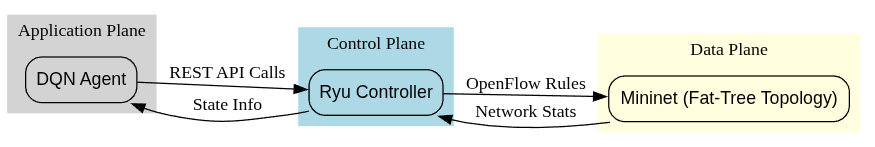
\includegraphics[width=0.8\linewidth]{Images/architecture_placeholder.png}
    \caption{DRL-SDN System Architecture}
\end{figure}
\end{frame}
\begin{frame}{Workflow of the Proposed Approach}
\begin{enumerate}
    \item Collect real-time network and server metrics
    \item Construct state representation
    \item Select action using DQN policy
    \item Enforce policy via OpenFlow rules
    \item Observe reward and next state
    \item Update DQN parameters
\end{enumerate}
\end{frame}
\begin{frame}{Network Topology}
\begin{figure}
    \centering
    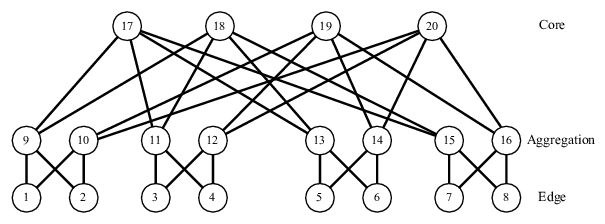
\includegraphics[width=0.75\linewidth]{Images/fat.png}
    \caption{Fat-Tree Topology (k = 4)}
\end{figure}
\end{frame}
\begin{frame}{MDP Formulation}
\begin{itemize}
    \item Problem modeled as Markov Decision Process
    \item Defined by $(\mathcal{S}, \mathcal{A}, \mathcal{R}, \gamma)$
    \item Enables sequential decision-making under uncertainty
\end{itemize}
\end{frame}

% ================= Frame 1: State =================
\begin{frame}{State Space}
\begin{block}{Server Metrics at Time $t$}
The agent observes the following vector of metrics for $S$ backend servers:
\[
\mathbf{s}_t = 
\big[
\text{cpu}_1, \text{memory}_1, \text{rtt}_1, \text{connections}_1, \text{requests}_1, \text{load\_score}_1, \;
\text{cpu}_2, \dots, \text{load\_score}_S
\big]
\]

\begin{itemize}
    \item $\text{cpu}_j$ = CPU usage of server $j$ (0--1)
    \item $\text{memory}_j$ = memory usage of server $j$ (0--1)
    \item $\text{rtt}_j$ = round-trip time to server $j$
    \item $\text{connections}_j$ = number of active connections
    \item $\text{requests}_j$ = total requests handled
    \item $\text{load\_score}_j$ = overall server load (0--1)
\end{itemize}
\end{block}
\end{frame}


% ================= Frame 2: Action =================
\begin{frame}{Action Space}
\begin{block}{Decision per Incoming Flow}
At each time step $t$, the agent selects a backend server for each incoming flow $f$:
\[
a_t : f \mapsto s_j, \quad s_j \in \{1, 2, \dots, S\}
\]

This action decides routing and load distribution across servers.
\end{block}
\end{frame}

% ================= Frame 3: Reward =================
\begin{frame}{Reward Design}
\begin{block}{Objective: Balanced Load and Low Latency}
The reward at time $t$ is computed from real server metrics:
\[
r_t = \underbrace{\alpha e^{- \text{avg RTT}/\tau_\text{RTT}}}_{\text{low latency}}
      + \underbrace{\beta e^{- \text{Var}(\ell_1,\dots,\ell_S)/\tau_\text{var}}}_{\text{balanced load}}
      + \underbrace{\text{balance bonus}}_{\text{even distribution}}
      - \underbrace{\text{overload penalty}}_{\text{avoid overloaded servers}}
\]

\begin{itemize}
    \item $\ell_j$ = server load, $j = 1\dots S$
    \item $\text{avg RTT} = \frac{1}{S}\sum_j rtt_j$
    \item $\text{Var}(\ell_1,\dots,\ell_S)$ = variance of server loads
    \item $\alpha, \beta$ = tunable reward weights
    \item Reward is clipped: $r_t \in [-10, 10]$
\end{itemize}
\end{block}
\end{frame}


\begin{frame}{DRL Agent Design}
\begin{itemize}
    \item Deep Q-Network (DQN)
    \item Online training with replay memory
    \item Target network for stability
    \item $\epsilon$-greedy exploration strategy
\end{itemize}
\end{frame}
\begin{frame}{Training Methodology}
\begin{itemize}
    \item Online interaction with SDN environment
    \item Transition storage in replay buffer
    \item Mini-batch gradient descent updates
    \item Periodic target network synchronization
\end{itemize}
\end{frame}
\begin{frame}{Hyperparameter Configuration}
\begin{itemize}
    \item State dimension: 18
    \item Action dimension: 3
    \item Hidden layer size: 64
    \item Learning rate: $3 \times 10^{-4}$
    \item Discount factor: 0.99
    \item Replay buffer size: 10,000
\end{itemize}
\end{frame}
\begin{frame}{Integration with Ryu Controller}
\begin{itemize}
    \item REST-based agent–controller communication
    \item Collection of port and flow statistics
    \item Dynamic flow rule installation
    \item Closed-loop learning and deployment
\end{itemize}
\end{frame}
\begin{frame}{Evaluation Metrics}
\begin{itemize}
    \item Throughput
    \item End-to-end latency
    \item Jain’s Fairness Index
    \item Link load variance
    \item Server CPU and memory utilization
\end{itemize}
\end{frame}
\begin{frame}{Tools Used}
\begin{itemize}
    \item Ryu Controller, Mininet, Open vSwitch
    \item Python, PyTorch, NumPy, Matplotlib
    \item Iperf, Apache Bench, Wireshark
    \item Arch Linux development environment
\end{itemize}
\end{frame}
